% FILE: figures/representation_flow_graph.tex
% Representation and information flow graph

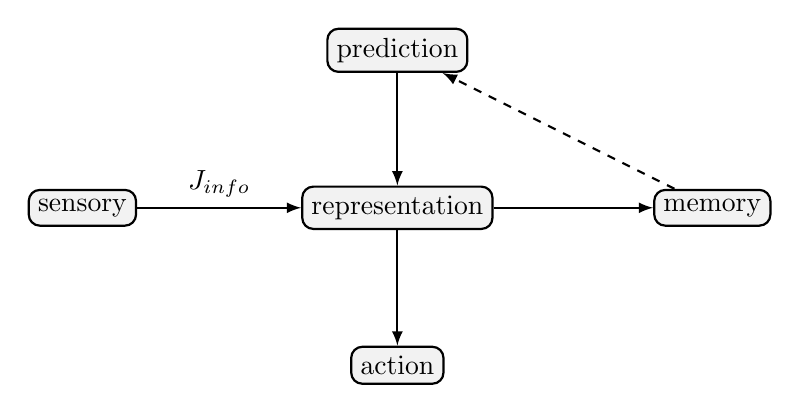
\begin{tikzpicture}[>=latex,thick,scale=1]
  % Nodes
  \node[draw, rounded corners, fill=gray!10] (Sens) at (0,0) {sensory};
  \node[draw, rounded corners, fill=gray!10] (Rep)  at (4,0) {representation};
  \node[draw, rounded corners, fill=gray!10] (Mem)  at (8,0) {memory};

  \node[draw, rounded corners, fill=gray!10] (Act)  at (4,-2) {action};
  \node[draw, rounded corners, fill=gray!10] (Pred) at (4,2) {prediction};

  % Edges
  \draw[->] (Sens) -- node[above] {$J_{\text{info}}$} (Rep);
  \draw[->] (Rep)  -- (Mem);
  \draw[->] (Rep)  -- (Act);
  \draw[->] (Pred) -- (Rep);
  \draw[->,dashed] (Mem) -- (Pred);
\end{tikzpicture}
